% TMS 2027 Annual Meeting & Exhibition -- proceedings manuscript (poster contribution)
% Accepted title (unqualified): From Transferability to Prediction: The Error Geometry of Interatomic Potentials
% Claim freeze: docs/plans/2026-09-09-tms-manuscript-sprint.md (binding). Every headline number is bound
% to a source row or frozen report in paper/tms2027-proceedings/results.json (built by build_artifacts.py).
\documentclass[11pt]{article}
\usepackage[T1]{fontenc}
\usepackage{lmodern}
\usepackage[letterpaper,margin=1in]{geometry}
\usepackage{amsmath,amssymb}
\usepackage{booktabs}
\usepackage{graphicx}
\usepackage{microtype}
\usepackage{array}
\usepackage{caption}
\usepackage{seqsplit}
\usepackage[hidelinks,breaklinks]{hyperref}
\usepackage[numbers,sort&compress]{natbib}
\hypersetup{
  pdftitle={From Transferability to Prediction: The Error Geometry of Interatomic Potentials},
  pdfauthor={Alex Welcing, Lupine Science}
}
\newcommand{\code}[1]{\texttt{#1}}
\newcommand{\fpath}[1]{\texttt{\seqsplit{#1}}}
\newcommand{\GPa}{\,\mathrm{GPa}}
\newcommand{\meV}{\,\mathrm{meV}}
\newcommand{\eV}{\,\mathrm{eV}}
\newcommand{\PR}{\mathrm{PR}}
\captionsetup{font=small,labelfont=bf}
\emergencystretch=3em

\title{From Transferability to Prediction:\\The Error Geometry of Interatomic Potentials}
\author{Alex Welcing\\Lupine Science\\\texttt{alex@lupinesci.com}\\ORCID \href{https://orcid.org/0009-0002-1602-8545}{0009-0002-1602-8545}}
\date{Proceedings manuscript for the TMS 2027 Annual Meeting \& Exhibition (poster). Draft of September 9, 2026.}

\begin{document}
\maketitle

\begin{abstract}
\noindent
Transferability is often summarized by a scalar error pooled across models, materials, and properties. We audit a vector alternative: the covariance geometry of errors in the three independent elastic constants of cubic metals. From 965 OpenKIM model objects queried, 559 mechanically admissible model--element tensors were retained across 15 elements; 42 potential groups covered at least three elements. These groups show strong descriptive anisotropy, with a median participation ratio of 1.09 out of 3. Registered stress tests, however, sharply limit the interpretation. Half of the 42 classical groups contain only three materials, which rank-limits a centered three-variable covariance; the classical analysis uses absolute errors whereas the foundation-model analysis uses relative errors; and cross-property participation-ratio and mode-alignment tests do not exceed coupling-aware nulls. After Born screening, classical alignment does not predict foundation machine-learning-potential alignment (Spearman correlation 0.26, $p=0.34$), while a global leave-one-out elastic correction increases mean error from 14.55 to 63.40 gigapascals. We therefore do not infer a universal hyper-ribbon or generally predictable transferability. The supported conclusion is narrower: error geometry is measurable only relative to a specified model family, observable, material class, and reference convention. We propose a qualification protocol combining vector residuals, stability gates, dependence-aware resampling, provenance-locked references, prospective prediction tests, and all-electron density-functional-theory anchors; the required elastic anchors remain pending.
\end{abstract}

\noindent\textbf{Keywords:} interatomic potentials; transferability; error measurement; elastic constants; model qualification

\section{Introduction}

Every finite-data model of atomic interactions is used outside the configurations it was calibrated on. Whether the model is a 1980s embedded-atom potential or a foundation machine-learning interatomic potential (MLIP) trained on millions of density-functional-theory (DFT) frames, its value to a materials engineer is set by how its error behaves under that transfer \citep{frederiksen2004,kurniawan2022,chiang2025mliparena}. Repositories such as OpenKIM and the NIST Interatomic Potentials Repository have made this question empirically tractable by fixing model identities, test protocols, and provenance for hundreds of potentials \citep{openkim,nist_ipr}. What the field still lacks is an agreed way to \emph{measure} transfer error as an object with structure, rather than a pooled scalar.

The sloppy-model literature offers a candidate structure. Multiparameter models generically have parameter sensitivities spanning many decades, so their model manifolds in prediction space are thin ``hyper-ribbons'' \citep{gutenkunst2007,transtrum2011,transtrum2015}; this spectrum has been documented for interatomic potentials directly \citep{frederiksen2004,wen2017,kurniawan2022} and for deep networks \citep{mao2024}. It is tempting to read the covariance of \emph{published-model} residuals as the same object and to promote a low participation ratio into a universality claim.

This paper reports what happened when we subjected exactly that reading to registered stress tests. The accepted poster abstract for this contribution described a universal hyper-ribbon that survives from classical potentials to MLIPs and makes transferability predictable. The record does not support that abstract, and this manuscript replaces it. Our contribution is a reference-, stability-, lineage-, and protocol-aware framework for measuring interatomic-potential error, together with a documented sequence of negative and conditional results obtained under it. The organizing thesis is:

\begin{quote}
In cubic-metal elasticity, prediction-error covariance is often anisotropic, but neither a universal hyper-ribbon nor a transferable correction axis is established. Transferability must therefore be qualified locally---by model family, observable, material class, reference convention, and data exposure---and tested prospectively with stability gates and independent DFT anchors.
\end{quote}

The paper is organized as four panels that mirror the poster: the denominator and provenance funnel (\S\ref{sec:funnel}); geometry under finite-sample and physical nulls (\S\ref{sec:geometry}); cross-paradigm and correction falsification (\S\ref{sec:falsification}); and the qualification protocol with its DFT-reference stack, in which the paired all-electron elastic anchor is a \emph{pending, preregistered} experiment rather than a result (\S\ref{sec:qualification}). Programs outside elasticity are summarized in one table (\S\ref{sec:other}) and are not pooled numerically with the elastic results.

\section{Error measurement: definitions}
\label{sec:definitions}

For model $i$, material $m$, property $k$, reference tier $r$, and protocol $p$, the signed residual is
\begin{equation}
e^{(r,p)}_{imk} = \frac{\hat y^{(p)}_{imk} - y^{(r,p)}_{mk}}{s^{(r,p)}_{mk}},
\label{eq:residual}
\end{equation}
where $s$ is a declared scale. We report at least two scales: absolute physical units (GPa), which carry decision relevance, and a preregistered dimensionless scale (relative error or reference uncertainty) for cross-property geometry. A participation ratio computed from absolute residuals is not comparable to one computed from relative residuals; this distinction matters below because the classical corpus was analyzed in GPa and the foundation-model corpus in relative error.

For a vector of residuals $e\in\mathbb R^d$ over an ensemble of models we separate three second-moment objects,
\begin{equation}
\mu = \mathbb E[e],\qquad C = \mathbb E[(e-\mu)(e-\mu)^{\!\top}],\qquad M = \mathbb E[ee^{\!\top}] = C + \mu\mu^{\!\top}.
\label{eq:moments}
\end{equation}
The centered covariance $C$ measures inter-model \emph{disagreement} geometry; $\mu$ measures shared signed \emph{bias}; the uncentered moment $M$ measures total quadratic risk and is the object required for any ``shared-bias fraction''. For a common reference, centered residuals satisfy $e_i-\bar e = \hat y_i - \bar{\hat y}$: the reference cancels. Centered principal-component analysis therefore cannot by itself establish accuracy, inherited DFT bias, or closeness to experiment. A previous inversion of the median centered participation ratio into ``about 98\% systematic error'' is withdrawn on these grounds.

The participation ratio of a spectrum $\{\lambda_j\}$ of $C$ is $\PR = (\sum_j\lambda_j)^2/\sum_j\lambda_j^2$, with $\PR\approx d$ for isotropic scatter and $\PR\approx k$ for scatter confined to $k$ dimensions \citep{transtrum2011}. Mechanical instability (violation of the Born conditions $C_{11}>0$, $C_{44}>0$, $C_{11}>|C_{12}|$), failed strain fits, and missing properties are treated as \emph{outcomes} and appear in the primary denominator; geometry is then reported conditionally among admissible tensors with a separate failure-rate endpoint. Every geometry statistic is to be compared with a matched null preserving the same $n$, $d$, missingness mask, marginal scales, elastic coupling and Born constraints, material and property families, and model lineage.

\section{Panel 1: the denominator and provenance funnel}
\label{sec:funnel}

Table~\ref{tab:funnel} and Fig.~\ref{fig:funnel} are the primary result of the classical corpus and replace every earlier statement of its size. All counts are recomputed from the committed data files by \code{build\_artifacts.py} and match the retained CSV row-for-row.

\begin{figure}[htbp]
\centering
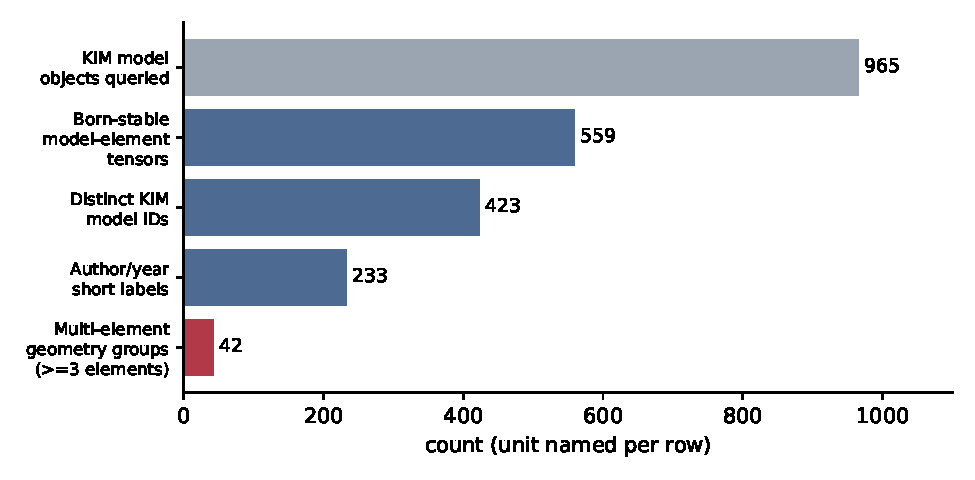
\includegraphics[width=0.85\textwidth]{figures/fig1_denominator_funnel.pdf}
\caption{Denominator and provenance funnel for the classical elastic corpus. Each bar is a different unit; the 42 analysis groups are groups of author/year short labels, not of KIM model identifiers (only 18 distinct identifiers cover three or more elements). Recomputed from \code{kim\_elastic\_results\_all.csv} and \code{manifold\_revalidation\_42potentials.json}.}
\label{fig:funnel}
\end{figure}

\begin{table}[htbp]
\centering
\caption{Denominator funnel for the classical cubic-metal elastic corpus. Each row names its unit; the units are not interchangeable. Sources: \code{kim\_elastic\_results\_all.csv}, \code{nist\_populated\_all.csv}, and \code{manifold\_revalidation\_42potentials.json} in the \code{lupine} repository.}
\label{tab:funnel}
\small
\begin{tabular}{@{}p{5.6cm}rp{6.6cm}@{}}
\toprule
Quantity & Count & Meaning \\
\midrule
KIM model objects queried & 965 & retrieval/search universe (OpenKIM query API) \\
Born-stable model--element tensors retained & 559 & analysis records; 356 fcc, 203 bcc; 15 elements \\
Distinct KIM model identifiers in the retained CSV & 423 & closest current model-object count \\
Author/year-style short labels & 233 & coarser labels that can merge model versions \\
Scalar $C_{ij}$ values & 1,677 & $559\times\{C_{11},C_{12},C_{44}\}$; dependent components \\
Multi-element geometry groups ($\geq3$ elements) & 42 & short-label groups in the committed revalidation file \\
\bottomrule
\end{tabular}
\end{table}

Three earlier descriptions of the same data are retired. ``Roughly 900 published potentials'' conflated the query universe with the retained records. ``559 independent potentials'' counted model--element tensors, of which only 423 carry distinct KIM identifiers and only 233 distinct author/year labels; the same parameterization contributes one tensor per element it was fitted for, so tensors are neither independent across elements nor unique to a publication. ``1,677 independent observations'' counted the three dependent components of each tensor. Within-tensor dependence also means that per-element correlations computed across $C_{11}$, $C_{12}$, and $C_{44}$ rows, and the Fisher-$z$ random-effects intervals previously built on them, are anti-conservative and are not reported here as inference.

Instability is itself an outcome. On the foundation-model side, the same Born screen applied to three pre-trained MLIPs (MACE-MP-0, CHGNet, Orb-v3 \citep{batatia2024,deng2023,rhodes2025}) on the same 15 elements rejected 7 of 45 element--model tensors, concentrated in bcc refractory metals; every model produced at least one unstable tensor out of the box. Alignment statistics for elements with an excluded model rest on a single surviving model pair.

\section{Panel 2: geometry under finite-sample and physical nulls}
\label{sec:geometry}

\subsection{Descriptive anisotropy}

Across the 42 committed groups, the participation ratio of the centered residual covariance in $(C_{11},C_{12},C_{44})$ ranges from 1.00 to 2.29 out of 3, with median 1.09 (Fig.~\ref{fig:pr}). The leading eigen-direction carries a median 96\% of centered variance. This is a genuine descriptive statement: within a family of parameterizations evaluated on several metals, the three elastic errors are far from isotropic. We keep it, and we keep the older classifier's label only as the descriptive phrase \emph{anisotropic elastic-error covariance}.

\begin{figure}[htbp]
\centering
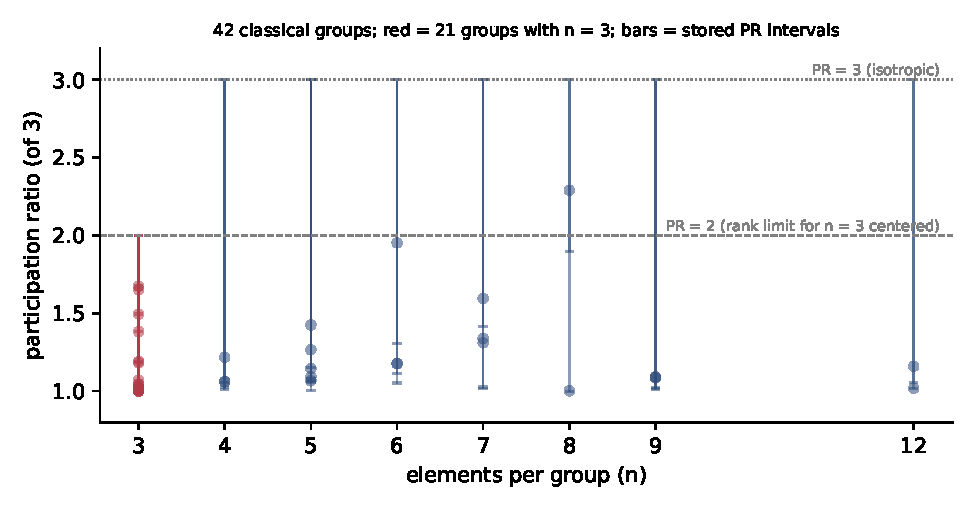
\includegraphics[width=0.9\textwidth]{figures/fig2_pr_vs_group_size.pdf}
\caption{Participation ratio against number of elements per group for the 42 classical groups. Red points are the 21 groups with exactly three elements; vertical bars are the stored bootstrap intervals. All 42 intervals reach at least $\PR=2$ and 21 reach approximately $\PR=3$. Source rows: \code{manifold\_revalidation\_42potentials.json}.}
\label{fig:pr}
\end{figure}

\subsection{Why the universality reading fails}

The committed 42-group file contains groups of 3, 4, 5, 6, 7, 8, 9, and 12 elements with counts 21, 3, 5, 3, 3, 2, 3, and 2. For the 21 groups with three elements, mean-centering three observations in a three-variable space forces the covariance to rank at most two; the stored spectra for all 21 indeed contain exactly two eigenvalues. A two-eigenvalue log spectrum is exactly linear, and a test for monotonic decay applied to already-sorted eigenvalues passes by construction. Half of the groups were therefore structurally predisposed to satisfy the hyper-ribbon classifier regardless of physics; their median $\PR$ is 1.03, against 1.16 for the 21 groups with four or more elements.

Uncertainty tells the same story. All 42 stored $\PR$ intervals reach at least 2, and 21 reach approximately 3, the isotropic value. The point estimate ``all 42 groups are low-dimensional'' is not an uncertainty-supported universality result. There is also a provenance gap: the stored monotonicity statistics do not match the current implementation for strictly descending spectra, and no committed generator reproduces the 42-group file from the CSV. The geometry recompute under absolute, relative, and standardized gauges with matched $n$/$d$/missingness/lineage nulls is a registered open item; until it clears the frozen null across strata, no strict hyper-ribbon claim is made.

Finally, the sloppy-model hyper-ribbon is a parameter-induced \emph{model manifold}; a covariance ellipsoid across published residuals is a different object and inherits none of the theorems that apply to the former. The retired claims from this panel are: universal hyper-ribbon or sloppy-model universality class; ``98\% systematic error'' from centered $\PR$; and causal bcc/fcc or $d$-band attribution, which an internal red-team found to be confounded by sampling depth, contamination, and reference composition.

\subsection{A live-ledger null test that is not yet reproducible}

The program's narrative record contains a pooled shared-stiffness signal, bounded to the elastic block, from a live-ledger snapshot of 352 rows. The snapshot, scripts, seeds, outputs, hashes, and refuter record had not been recovered intact at the time of writing. Following the sprint contract, its exact participation-ratio, null, and correction numbers are omitted here rather than quoted from narrative. If they are recovered, they belong in the same canonical results object as the numbers in this paper.

\section{Panel 3: cross-paradigm and correction falsification}
\label{sec:falsification}

\subsection{Classical alignment does not predict foundation-model alignment}

For each element we computed the cosine alignment of leading error directions between distinct classical functional-form families and, separately, the pairwise cosine alignment among the Born-stable foundation-model error vectors. The two per-element orderings are unrelated: Spearman $\rho=0.26$, $p=0.34$ over 15 elements. Elements with strong classical alignment (Ta, Nb, Au, Ag, Cr, Pb, Pt) have mean MLIP cosine 0.52, while the weak-classical set (Pd, Al, W, Fe) has 0.68. Directional structure exists in both paradigms for most elements, but it is paradigm-specific: the classical grouping has no predictive power for the MLIP grouping. With three foundation models per element, a participation-ratio test is not meaningful (three centered vectors span at most two dimensions), so no cross-paradigm dimensionality claim is made. The retired statement is ``the hyper-ribbon survives 14 of 15 metals from classical to MLIP''.

\subsection{Functional and cross-property tests}

A registered $4\times2$ MatPES study (four foundation architectures, PBE and r$^2$SCAN training labels, 16 cubic metals) tested whether error vectors cluster by exchange-correlation functional rather than by architecture. Both primary kill conditions fired: the functional-clustering effect size on the 3$d$/4$d$ subset was $-0.14$ (same-architecture pairs aligned more closely than same-functional pairs) and the permutation $p$ was 0.13. An initial functional-label association therefore did not survive the stricter Round-2 protocol, and no causal exchange-correlation attribution is made. The four MatPES models share training data and are not four independent architectures for the purpose of an ensemble-independence claim.

A separate preregistered cross-property study (57 GPU cells: 19 materials $\times$ MACE-MP-small, MACE-MP-medium, CHGNet; 345 reference-bound properties spanning lattice constant, bulk modulus, vacancy formation, and surface energies) asked whether low dimensionality extends across property families. Under a coupling-aware null that preserves within-family magnitude structure, low dimensionality was not confirmed in 4 of 6 tests, and no shared leading error mode survived in 3 of 3 model-pair tests: raw mode cosines reached 0.96, but the null's 95th percentile reached 0.98. A naive analysis would have reported both as confirmation. The one effect that did replicate across every model and both matrices---defect-family errors 15--57 times bulk-family errors---is the published softening pathology of MPtrj-trained potentials \citep{deng2025softening} measured on this instrument, and it argues for family-targeted rather than global correction.

\subsection{Global correction: a prospective failure and an oracle ceiling}

Figure~\ref{fig:correction} separates two results that have been conflated.

\begin{figure}[htbp]
\centering
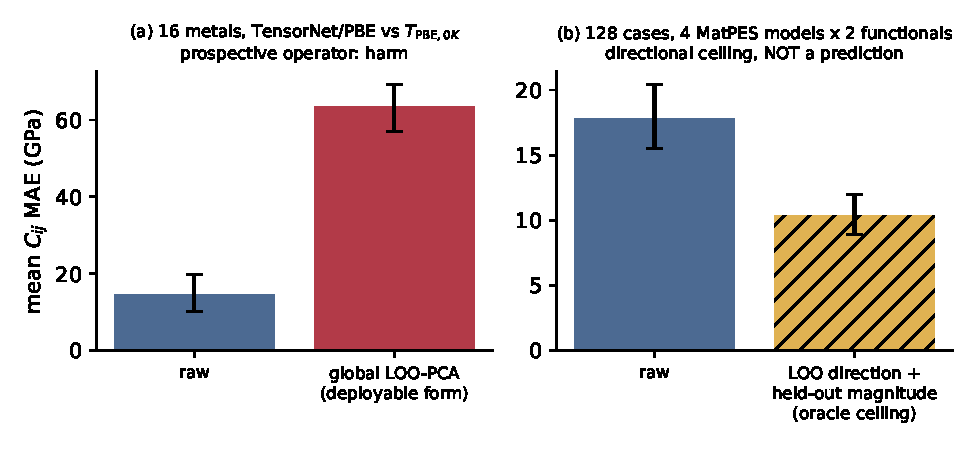
\includegraphics[width=0.95\textwidth]{figures/fig3_correction_arms.pdf}
\caption{Two different correction statements on two different benchmarks. (a) A deployable global leave-one-out principal-component operator, fitted on 15 held-in metals and applied to the held-out metal, increases mean $C_{ij}$ MAE from 14.55 to 63.40 GPa (bootstrap 95\% intervals $[10.08,19.72]$ and $[57.07,69.18]$); it worsens all 16 metals. Source: hash-locked \code{global-operator.lock.json}. (b) On the 128-case MatPES benchmark, projecting the held-out residual onto a leave-one-out direction \emph{with the held-out target supplying the coefficient} lowers mean MAE from 17.84 to 10.36 GPa. This is an oracle directional ceiling, not a prediction. The two panels use different models, targets, and estimands and must not be read as one operator.}
\label{fig:correction}
\end{figure}

The prospective result is the failure. On a 16-metal cubic benchmark (TensorNet/PBE predictions against curated 0\,K PBE targets), the v0.1 global leave-one-out principal-component operator increased mean $C_{ij}$ MAE from $14.55\GPa$ to $63.40\GPa$ and worsened every one of the 16 elements. Leave-one-out fitting prevents direct target leakage, but it cannot make a single global error direction transferable when element-level error directions differ. The failure was reproduced in an independent 2026-07-13 re-execution to within $0.01\GPa$.

The oracle result is the ceiling. On the 128-case benchmark (16 metals, four MatPES models, PBE and approximate r$^2$SCAN targets; raw mean $C_{ij}$ MAE $17.84\GPa$, 95\% CI $[15.51,20.41]$), extracting a per-functional bias direction from the other 63 same-functional cases and projecting the held-out residual onto it lowers mean MAE to $10.36\GPa$ (95\% CI $[8.9,12.0]$) with no held-out row worsened. That procedure uses the held-out target to set the projection magnitude. It measures how much residual energy a training-derived \emph{direction} can capture; it is not a target-free prediction and does not license deployment. The same distinction applies to the associated ``69\% of residual energy captured'' figure. Required comparators for any future deployable claim are raw prediction, mean or family shift, diagonal or ridge baselines, a random basis, and abstention, with both mean improvement and number of cases harmed reported.

Two further preregistered rounds tested a frozen, abstaining, same-class ratio correction on held-out ionic rocksalt and perovskite candidates (four models each). In Round 3 the rule improved same-class lattice constants (median relative error 1.60\%$\to$0.33\% for rocksalts and 1.75\%$\to$0.74\% for perovskites, sign-test $p=3\times10^{-5}$) while worsening or abstaining on every elastic property; both groups failed the registered two-thirds property-win criterion and the registered kill fired, narrowing the public correction scope to same-class lattice constants. Round 4, with a theorem-derived magnitude cap, recorded zero confirmatory property wins (0/4 rocksalt, 0/1 perovskite). The retired statements are ``deployable correction'', ``unconditional no-harm'', and any prediction based on $17.84\to10.36\GPa$.

\section{Panel 4: qualification protocol and the DFT-reference stack}
\label{sec:qualification}

\subsection{Reference taxonomy}

We distinguish three tiers that were previously blurred (Fig.~\ref{fig:stack}). \emph{Prediction controls} are completed model outputs (MACE, CHGNet, Orb, MatPES models); they are not truth. \emph{Reference targets} are literature DFT or experiment; they may be mixed, approximate, finite-temperature, or convention-mismatched. \emph{Computed ab-initio anchors} are new calculations under one frozen protocol with raw outputs and convergence evidence. A qualification statement about a potential must name the tier of every number it compares against.

\begin{figure}[htbp]
\centering
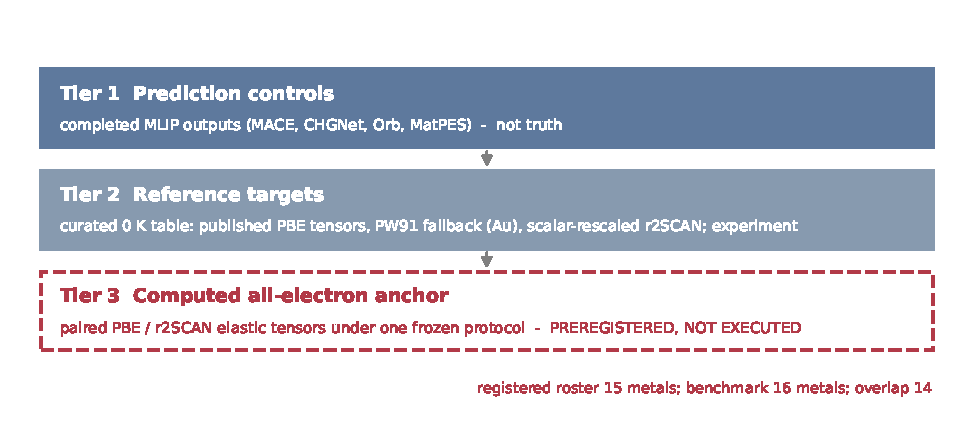
\includegraphics[width=0.9\textwidth]{figures/fig4_reference_stack.pdf}
\caption{The DFT-reference stack. Solid tiers exist in the record; the dashed tier---the paired all-electron PBE/r$^2$SCAN elastic anchor---is preregistered and has not been executed. Its registered 15-metal roster and the completed 16-metal benchmark overlap on 14 metals.}
\label{fig:stack}
\end{figure}

Under this taxonomy the completed 16-metal, 128-case benchmark measures MLIP discrepancy against a curated 0\,K target table comprising mostly published PBE tensors, a PW91 fallback for Au, and approximate scalar-rescaled r$^2$SCAN targets (a $+5.65\GPa$ mean gap between functionals). Because the r$^2$SCAN targets are PBE tensors scaled by a bulk-modulus ratio, any operator that improves agreement with them is partly aligned with the target by construction.

\subsection{The all-electron elastic anchor: pending}

The decomposition of fitting error from functional and reference-standard offsets requires a paired all-electron PBE/r$^2$SCAN elastic-constant anchor computed under one protocol. This experiment is preregistered (\code{prereg\_r2b\_dft\_anchor\_spec.md}) and has \emph{not} been executed. Its registered roster is the 15-metal set (Al, Cu, Ni, Ag, Au, Pt, Pd, Pb; Fe, Cr, Mo, W, V, Nb, Ta), while the completed benchmark covers a 16-metal set including Ca and Sr and excluding Pb; the two overlap on 14 metals. The expected result files do not exist; the staged runner depends on an uncommitted script; the convergence record and the planned LAPW cross-check are absent; magnetic ordering, starting moments, and exclusion rules are not operationally frozen; and the available all-electron equation-of-state comparisons cover $(V_0,B_0,B_1)$ rather than $(C_{11},C_{12},C_{44})$. We therefore describe it as the closing experiment of the protocol, not as a result. The retired statement is ``all-electron elastic anchor completed''.

\subsection{The protocol}

The qualification protocol that the evidence above supports has six components, each tied to a failure it prevents.
\begin{enumerate}
\item \textbf{Vector residuals on declared scales} (Eq.~\ref{eq:residual}), reported in both GPa and a preregistered dimensionless gauge, so that geometry across observables and paradigms is compared like with like.
\item \textbf{Stability and harness failures as endpoints}, in the primary denominator, so that admissibility filtering cannot silently improve a corpus.
\item \textbf{Dependence-aware resampling and matched nulls}: block resampling over model lineage and material; nulls that preserve $n$, $d$, missingness, coupling, Born constraints, and families. The Y-matrix test shows this is not optional: a 0.96 cosine was inside a 0.98 null.
\item \textbf{Provenance-locked references}: every target row carries its tier, functional, temperature, and convention, and the results object is hash-locked to the source rows (this paper's \code{results.json} records the SHA-256 of each source).
\item \textbf{Prospective prediction tests}: hold out the full deployment unit (a model lineage and/or a material); learn normalization, basis, coefficient estimator, gates, and hyperparameters inside the training fold; report raw, shift, ridge, random-basis, and abstention baselines with mean improvement and number harmed.
\item \textbf{Computed all-electron anchors} under one frozen protocol, to separate fitting error from functional and reference offsets---pending for elasticity, as stated above.
\end{enumerate}
``Prediction'' in the title is the endpoint of this protocol, not a result already achieved.

\section{Programs outside elasticity}
\label{sec:other}

Table~\ref{tab:other} summarizes four programs that inform the protocol but are not pooled numerically with the elastic results; they differ in observable, chemistry, model set, correction form, and reference tier.

\begin{table}[htbp]
\centering
\caption{Non-elastic programs, kept separate. Defensible and non-defensible statements are taken verbatim from the frozen program status; numbers are quoted from the named hash-locked records and are not combined with any elastic quantity.}
\label{tab:other}
\small
\setlength{\tabcolsep}{4pt}
\begin{tabular}{@{}p{2.2cm}p{5.2cm}p{4.2cm}p{3.6cm}@{}}
\toprule
Program & Defensible now & Not defensible & Record \\
\midrule
Li migration barriers (Z1) & Four foundation MLIPs fail a preregistered $40\meV$ DFT-NEB gate on 30 chemistry-held-out paths: float64 MAE $135.0$--$242.5\meV$ over 26--29 completed paths. Sign imbalance is model-dependent (negative errors 25/28 CHGNet, 21/29 MACE-MP-medium, 17/26 MACE-MP-small, 13/28 MACE-MPA-0). & ``Every completed path underpredicts''; universal barrier underprediction. & negative-results preprint, hash-locked Z1 chain \citep{dembitskiy2025litraj} \\
Sparse barrier anchors & 129 GPAW anchor points on 23 short paths establish sparse-vs-dense reconstruction \emph{within the same engine}; guidance quality ranks models (two models located every extremum). Seven long paths deferred. & External DFT accuracy, ``DFT-grade'' accuracy, or a realized prospective savings claim; GPAW--VASP convention wander ($\sim$1\,eV mean) prevented external validation. & \fpath{z1-union-campaign-verdict.md} \\
Adsorption $\Delta$-correction (Z3) & 128/128 CatBench baseline cells completed; a frozen 6/6/20 train/validation/test protocol worsened untouched holdout MAE for all four models ($0.69\to2.27$, $2.11\to5.01$, $3.24\to5.00$, $4.27\to5.91\eV$). & General $\Delta$-correction efficacy from the frozen small-budget design. & negative-results preprint \citep{catbench2025dataset,pablogarcia2023gamenet} \\
Environment error field & Blind coordination-field prediction of $\gamma_{110}$ attains $r=0.906$ over 36 (model, material) cells; a nonlinear alternative to a global linear ribbon. & Generalization beyond the tested fcc/mixed-reference scope; force-level correction without external replication. & \fpath{environment-error-field-2026-07-02.md} \\
Formal (Lean 4) layer & Conditional algebra of corrections, failure boundaries, and claim contracts are machine-checked (899 theorem/lemma declarations across 111 modules, zero \code{sorry}, count generated 2026-08-08). & Empirical validation of any theorem hypothesis, or ``proof'' that a physical correction works; a prior gate was found not to be licensed by the theorem it cited. & \fpath{lean-spec/theorem-count.json}; errata 2026-07-13 \\
\bottomrule
\end{tabular}
\end{table}

\section{Discussion}

The program set out to find a universal law and found, instead, that attractive low-dimensional and correction claims can disappear under better denominators, physical stability gates, coupling-aware nulls, genuinely held-out tests, and independent reference checks. We regard that self-correction as the result. Three lessons generalize beyond cubic metals.

First, the unit of a sample size is part of the claim. ``Potential'', ``model identifier'', ``parameterization'', ``lineage'', ``model--element tensor'', and ``elastic-constant component'' are six different denominators for one CSV, and inference changes by an order of magnitude depending on which is chosen. Second, geometry needs a physics-preserving null. Centering removes the reference and rank-limits small groups; elastic coupling and Born constraints induce correlations that a shuffled or Gaussian null does not reproduce. The Y-matrix experiment, in which a 0.96 cosine fell inside a 0.98 null, is the clearest demonstration in our record. Third, a correction earns its scope out of sample or not at all. The oracle ceiling ($17.84\to10.36\GPa$) and the prospective failure ($14.55\to63.40\GPa$) are answers to different questions; only the second is about deployment, and it says the global direction is harmful.

What remains defensible is narrower than the accepted abstract but, we think, more useful: a measurable, provenance-locked description of anisotropic elastic-error covariance; a set of registered negative results that rule out the simplest universal explanations; and a qualification protocol whose closing experiment---the paired all-electron elastic anchor---is specified and pending.

\section*{Data and code availability}

All numbers in this manuscript are bound to source rows or frozen reports in \fpath{paper/tms2027-proceedings/results.json}, generated by \fpath{paper/tms2027-proceedings/build\_artifacts.py} in the \code{lupine-rhizo} repository (\url{https://github.com/alexwelcing/lupine-rhizo}); the script records the SHA-256 of every source file and fails closed on drift, and \code{--check} verifies that the committed results object is current. The classical corpus (\code{kim\_elastic\_results\_all.csv}, 559 rows; \code{nist\_populated\_all.csv}, 1,677 rows), the 42-group geometry file, the MatPES benchmark summary, and the all-electron anchor preregistration are in \url{https://github.com/alexwelcing/lupine}; the replication kit snapshot is archived at \url{https://doi.org/10.5281/zenodo.20787874}. The global-operator lock, Z1 and Z3 chains, Round-3/4 reports, and the Y-matrix analysis artifacts are in \code{lupine-rhizo} with SHA-256 sidecars. Raw classical predictions were obtained from the OpenKIM query API \citep{openkim} and cross-referenced with the NIST Interatomic Potentials Repository \citep{nist_ipr}; experimental references are from Simmons and Wang \citep{simmons1971}. The 352-row live-ledger snapshot referenced in \S\ref{sec:geometry} had not been recovered at submission and no numbers from it appear here.

\section*{Use of AI assistance}

AI assistants (Anthropic Claude, OpenAI Codex, and others) were used under the author's direction for recomputation, consistency checking of manuscript claims against the committed data, adversarial internal review, and language editing. All scientific claims and interpretations were reviewed by the author, who takes sole responsibility for the content.

\section*{Acknowledgments}

The author thanks the OpenKIM consortium and the NIST Interatomic Potentials Repository for maintaining the provenance infrastructure that made the denominator audit possible, and the hostile-referee reviewers whose 2026-07-13 dispositions are reflected throughout.

\bibliographystyle{unsrtnat}
\bibliography{references}

\end{document}
